% This file was created with tikzplotlib v0.10.1.
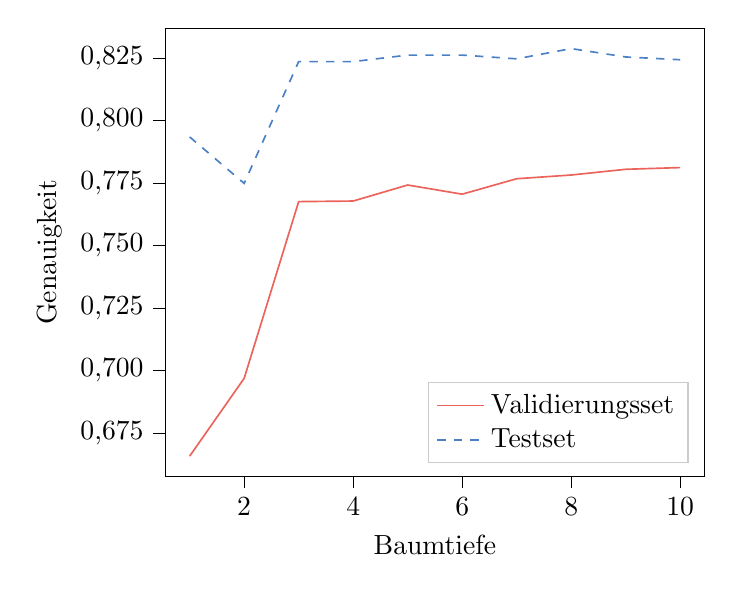
\begin{tikzpicture}

\definecolor{darkgray176}{RGB}{176,176,176}
\definecolor{lightgray204}{RGB}{204,204,204}
\definecolor{steelblue75129196}{RGB}{75,129,196}
\definecolor{tomato2369992}{RGB}{236,99,92}

\begin{axis}[
legend cell align={left},
legend style={
  fill opacity=0.8,
  draw opacity=1,
  text opacity=1,
  at={(0.97,0.03)},
  anchor=south east,
  draw=lightgray204
},
tick align=outside,
tick pos=left,
x grid style={darkgray176},
xlabel={Baumtiefe},
xmin=0.55, xmax=10.45,
xtick style={color=black},
y grid style={darkgray176},
ylabel={Genauigkeit},
ymin=0.657595009157509, ymax=0.837024954212454,
ytick style={color=black},
ytick={0.65,0.675,0.7,0.725,0.75,0.775,0.8,0.825,0.85},
yticklabels={{0,650},{0,675},{0,700},{0,725},{0,750},{0,775},{0,800},{0,825},{0,850}}
]
\addplot [semithick, tomato2369992]
table {%
1 0.665750915750916
2 0.696886446886447
3 0.767628205128205
4 0.767857142857143
5 0.774267399267399
6 0.770604395604396
7 0.776785714285714
8 0.77827380952381
9 0.780563186813187
10 0.78125
};
\addlegendentry{Validierungsset}
\addplot [semithick, steelblue75129196, dashed]
table {%
1 0.793526785714286
2 0.774925595238095
3 0.823660714285714
4 0.823660714285714
5 0.826264880952381
6 0.826264880952381
7 0.824776785714286
8 0.828869047619048
9 0.825520833333333
10 0.824404761904762
};
\addlegendentry{Testset}
\end{axis}

\end{tikzpicture}
